% =====================================================================
% SECTION 4 - EMULADOR ESTOCASTICO DEPENDENTE DO TEMPO (GLaM)
% Traducao e reorganizacao do arquivo GLaM_Marcos.tex, acrescida da
% subsecao de metricas de validacao (KS, AD, KL e quantis), que estava
% dispersa na antiga Section_2/Section_4.
% =====================================================================

O elevado custo computacional de modelos de alta fidelidade frequentemente inviabiliza simulações diretas de Monte Carlo, exigindo o uso de metamodelos, também chamados de emuladores. Embora Processos Gaussianos (GP) \citep{rasmussen2006} e Expansões em Caos Polinomial (PCE) \citep{xiu2002} sejam padrão para sistemas determinísticos, eles não podem ser aplicados diretamente a simuladores estocásticos, nos quais uma única avaliação é insuficiente para caracterizar a distribuição da resposta.

\subsection{Simuladores estocásticos}
\label{subsec:simulador}

Matematicamente, um simulador estocástico $\mathcal{M}_S$ pode ser visto como um mapeamento que incorpora variáveis determinísticas e aleatoriedade intrínseca. Para um dado vetor de parâmetros de entrada $\mathbf{x}$ no domínio $\mathcal{D}_X$, a resposta não é um valor determinístico único, mas uma variável aleatória $Y_{\mathbf{x}}$. Essa relação é formalmente expressa como:

\begin{equation}
\mathcal{M}_S : \mathcal{D}_X \times \Omega \rightarrow \mathbb{R}, \qquad (\mathbf{x}, \omega) \mapsto \mathcal{M}_S(\mathbf{x}, \omega),
\label{eq:simulador_estocastico}
\end{equation}

\noindent em que $\mathbf{x}$ representa o conjunto de parâmetros de entrada controlados (e.g., geometria, propriedades dos materiais) e $\omega$ denota um evento aleatório do espaço de probabilidade $\Omega$. Essa variável latente $\omega$ introduz a estocasticidade no sistema. Consequentemente, para uma entrada fixa $\mathbf{x}$, o simulador produz uma distribuição de resultados possíveis, e não uma solução única. No problema em estudo, $\mathcal{M}_S(\mathbf{x}, \omega) = g(\mathbf{x}, t; \omega)$ é a função de estado limite definida na Equação~\eqref{eq:funcao_g}, e as variáveis latentes correspondem às incertezas de modelo e às flutuações não explicitamente parametrizadas.

\subsection{Distribuição Lambda Generalizada}
\label{subsec:gld}

No contexto da avaliação de durabilidade do concreto armado, o processo de carbonatação é influenciado por diversas fontes de incerteza, que vão da heterogeneidade do material às flutuações ambientais. Para capturar esses comportamentos probabilísticos complexos sem o custo computacional de simulações exaustivas, este estudo emprega a Distribuição Lambda Generalizada (GLD) como núcleo do emulador estocástico. A GLD é uma família de distribuições de quatro parâmetros, altamente flexível, projetada para aproximar uma ampla gama de distribuições paramétricas \citep{KarianDudewicz2000, ZhuSudret2021}.

A GLD é definida por sua \textit{função quantílica} $Q(u)$, que é a inversa da função de distribuição acumulada (CDF), i.e., $Q(u) = F^{-1}(u)$. Essa abordagem é particularmente vantajosa para a emulação estocástica, pois facilita o método de amostragem por transformada inversa. Neste estudo, considera-se a família Freimer--Kollia--Mudholkar--Lin (FKML) \citep{Freimer1988}, definida como:

\begin{equation}
Q(u) = \lambda_1 + \frac{1}{\lambda_2} \left( \frac{u^{\lambda_3} - 1}{\lambda_3} - \frac{(1 - u)^{\lambda_4} - 1}{\lambda_4} \right)
\label{eq:GLD_quantile}
\end{equation}

\noindent em que $u \in [0, 1]$ representa a probabilidade acumulada. A distribuição é governada por quatro parâmetros: $\lambda_1$ é o parâmetro de \textit{locação}, $\lambda_2$ é o parâmetro de \textit{escala} (com a exigência $\lambda_2 > 0$) e $\lambda_3, \lambda_4$ são os parâmetros de \textit{forma}.

\subsection{Estimação de parâmetros via método dos momentos}
\label{subsec:mom}

Para calibrar o emulador GLD, os quatro parâmetros $\boldsymbol{\lambda} = \{\lambda_1, \dots, \lambda_4\}$ devem ser estimados a partir de um conjunto de avaliações do modelo \citep{karian2010handbook, corlu2016}. Neste estudo, emprega-se o \textit{Método dos Momentos} (MoM) \citep{lakhany2000}, que consiste em igualar os momentos teóricos da GLD aos momentos empíricos calculados do conjunto amostral $\mathcal{Y} = \{y^{(1)}, \dots, y^{(N)}\}$. Os quatro primeiros momentos centrais --- média $\mu$, variância $\sigma^2$, assimetria $\delta$ e curtose $\kappa$ --- relacionam-se analiticamente aos parâmetros $\lambda$ da seguinte forma:

\begin{align}
\mu &= \lambda_1 - \frac{1}{\lambda_2} \left( \frac{1}{\lambda_3 + 1} - \frac{1}{\lambda_4 + 1} \right) \label{eq:mean} \\
\sigma^2 &= \frac{v_2 - v_1^2}{\lambda_2^2} \label{eq:var} \\
\delta &= \frac{v_3 - 3v_1v_2 + 2v_1^3}{(v_2 - v_1^2)^{3/2}} \label{eq:skew} \\
\kappa &= \frac{v_4 - 4v_1v_3 + 6v_1^2v_2 - 3v_1^4}{(v_2 - v_1^2)^2} \label{eq:kurt}
\end{align}

Nessas expressões, $v_k$ denota uma função não linear que depende apenas de $\lambda_3$ e $\lambda_4$, dada pela Equação~\eqref{eq:vk}, em que $B(\cdot, \cdot)$ representa a função Beta:

\begin{equation}
v_k = \sum_{j=0}^{k} \frac{(-1)^j}{\lambda_3^{k-j} \lambda_4^j} \binom{k}{j} B\!\left(\lambda_3(k-j) + 1,\; \lambda_4 j + 1\right) \label{eq:vk}
\end{equation}

A calibração dos parâmetros da GLD é formulada como um problema inverso, cujo objetivo é minimizar a discrepância entre os momentos analíticos (Equações~\ref{eq:mean}--\ref{eq:kurt}) e os momentos empíricos derivados do simulador estocástico. Para resolver esse sistema não linear, emprega-se o algoritmo de otimização Broyden--Fletcher--Goldfarb--Shanno (BFGS) \citep{nocedal2006}, um método quase-Newton particularmente adequado a esse tipo de estimação devido ao tratamento eficiente de gradientes e às boas propriedades de convergência em espaços multidimensionais. O procedimento numérico foi implementado no PyGLAM, biblioteca Python desenvolvida pelos autores especificamente para a emulação de simuladores estocásticos com Distribuições Lambda Generalizadas.

Cabe registrar que o arcabouço GLaM original \citep{ZhuSudret2021} emprega máxima verossimilhança condicional combinada a mínimos quadrados generalizados para a estimação dos parâmetros, dispensando réplicas no plano de experimentos. A opção pelo MoM com réplicas adotada neste trabalho justifica-se (i) pela robustez e simplicidade de implementação, (ii) pelo baixo custo de cada avaliação dos modelos mecânicos aqui considerados, que torna as réplicas viáveis, e (iii) pelo controle direto da qualidade do ajuste local em cada ponto do plano de experimentos, requisito importante para a camada temporal descrita na Seção~\ref{subsec:temporal}.

A Figura~\ref{fig:pyglam_fits} apresenta exemplos de ajuste da GLD a distribuições tradicionais --- Normal, Gumbel e Uniforme --- obtidos com o PyGLAM, e a Tabela~\ref{tab:pyglam_metricas} quantifica a qualidade desses ajustes. \falta{preencher a tabela com distância de Wasserstein, estatística KS e erro relativo nos quantis P5/P50/P95 para cada distribuição-alvo, variando o tamanho amostral (ex.: $N$ = 50, 200, 1000)}

\begin{figure}[htbp]
     \centering
     \begin{subfigure}[b]{0.32\textwidth}
         \centering
         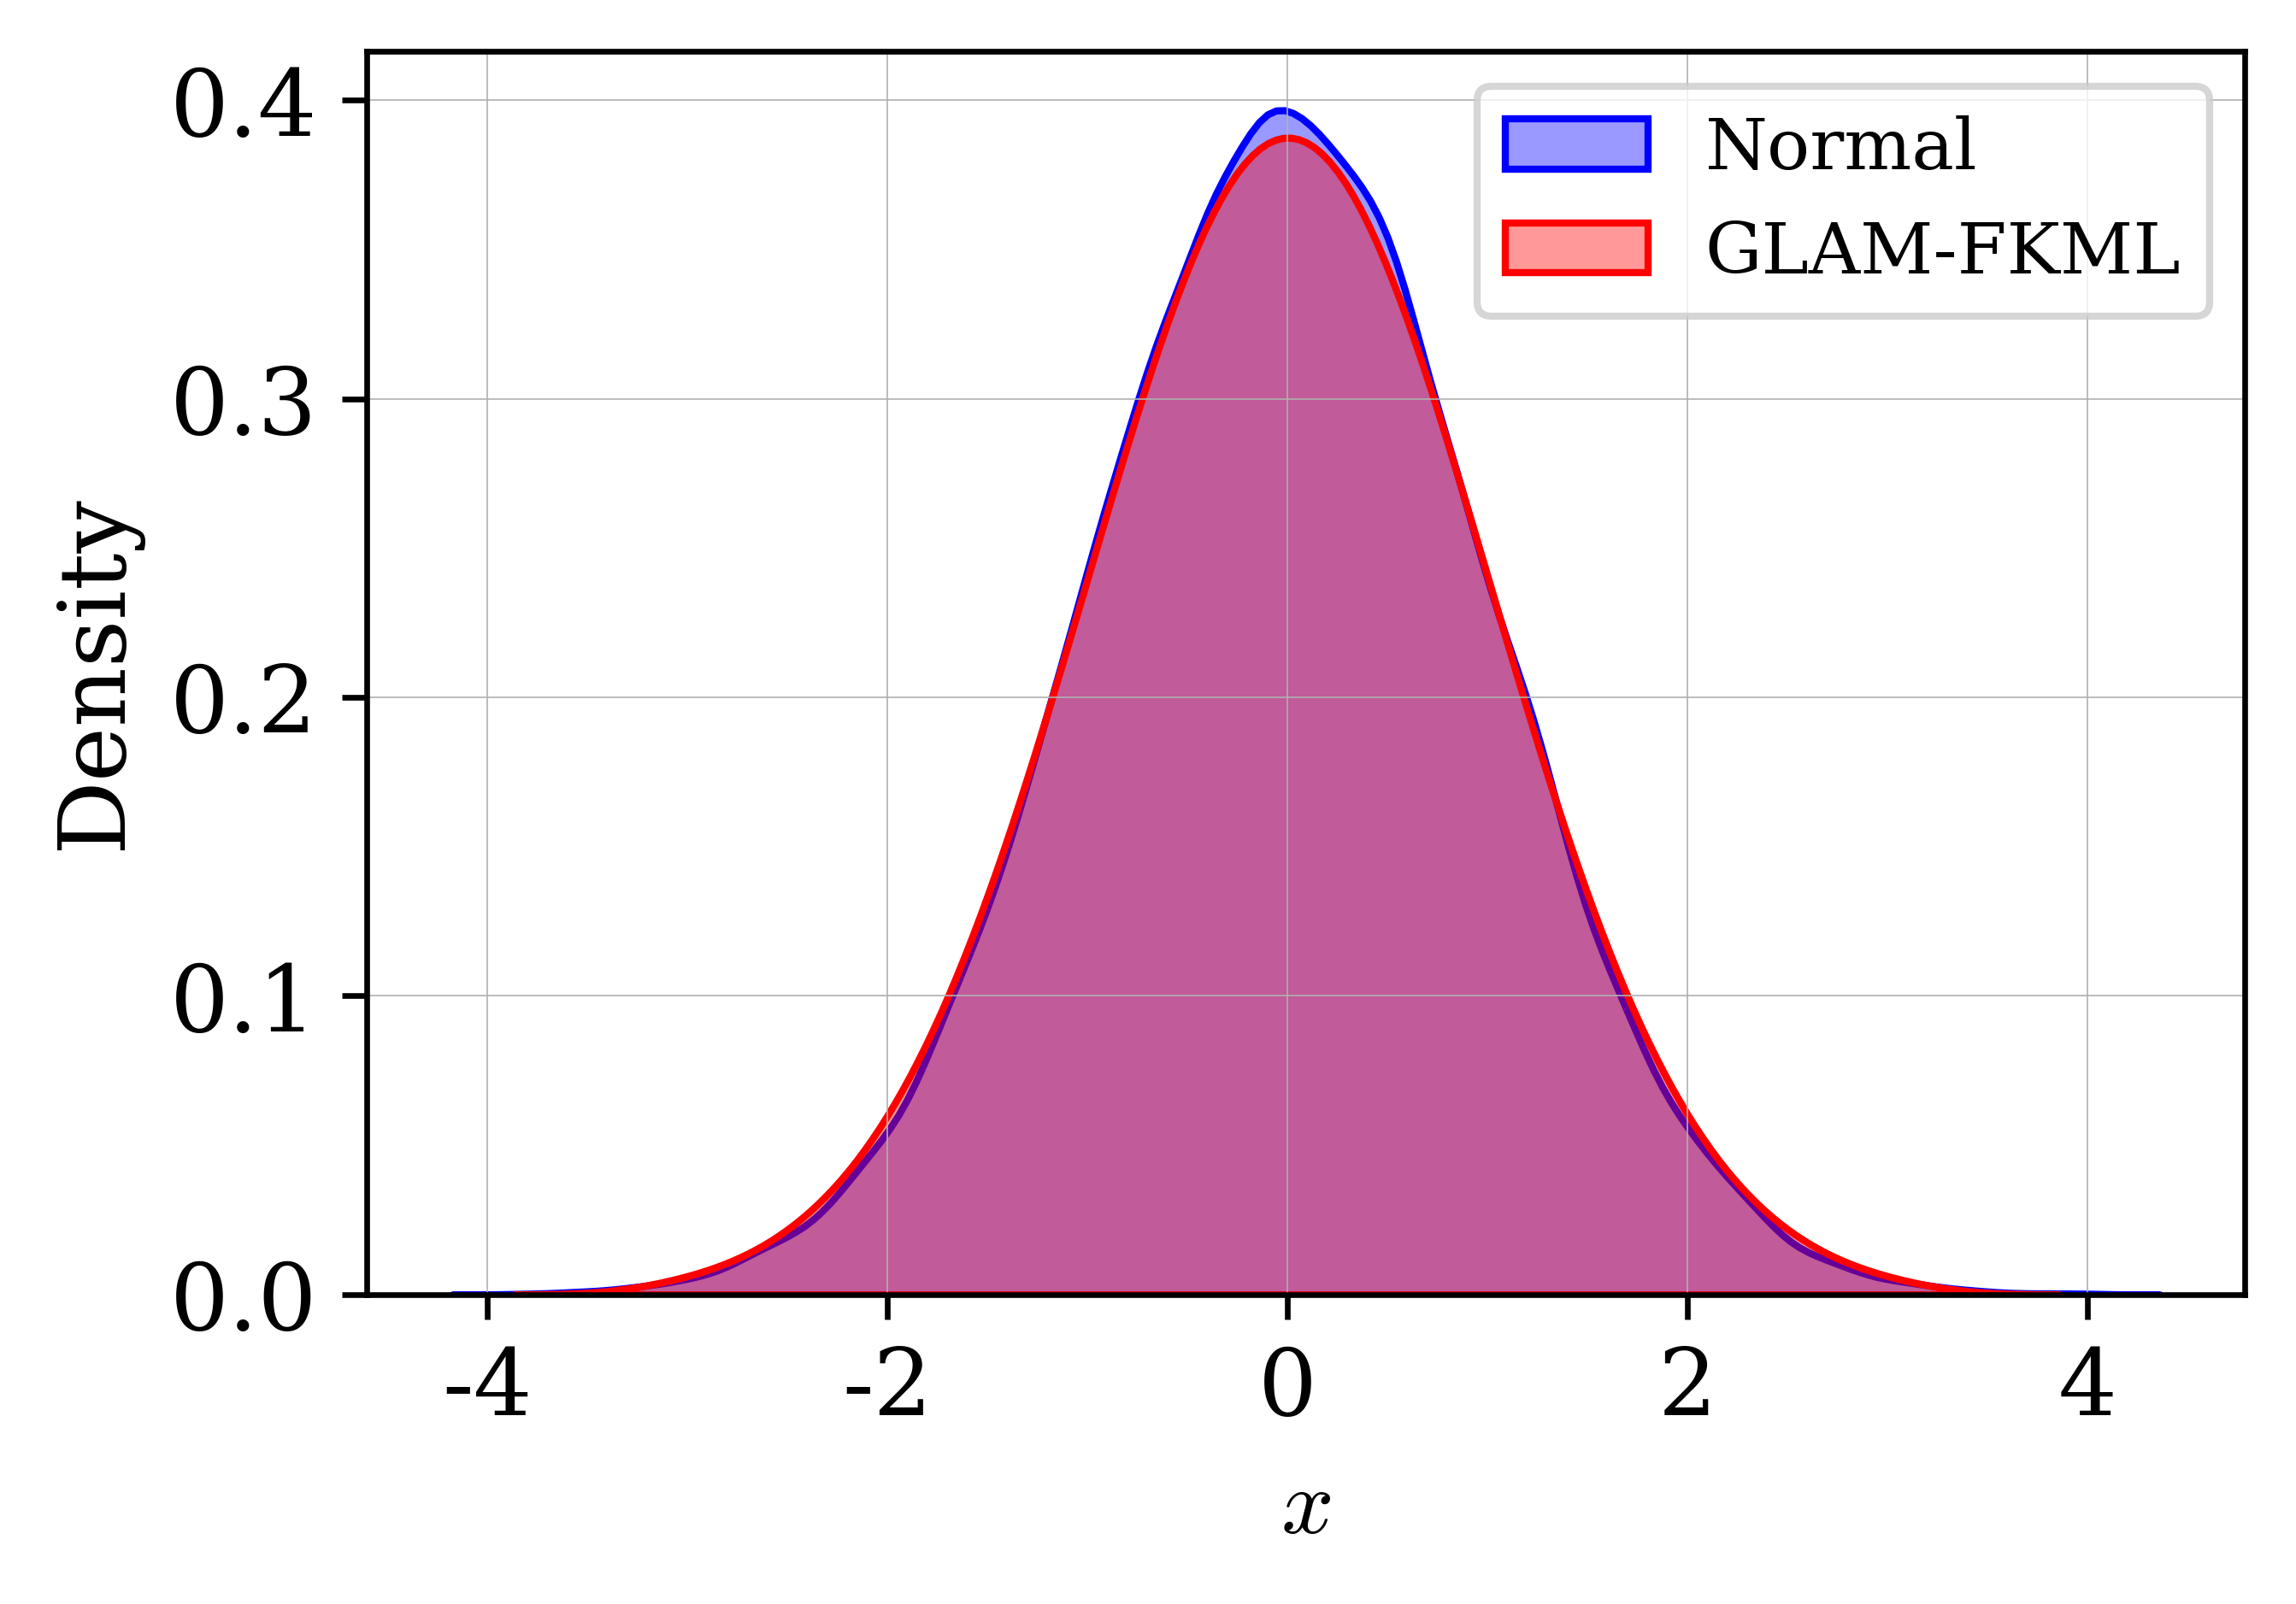
\includegraphics[width=\textwidth]{z_kde_histogram_compare.png}
         \caption{Distribuição Normal}
         \label{fig:fit_normal}
     \end{subfigure}
     \hfill
     \begin{subfigure}[b]{0.32\textwidth}
         \centering
         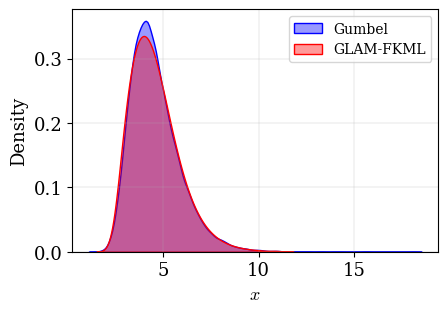
\includegraphics[width=\textwidth]{z_fig_gumbel.png}
         \caption{Distribuição de Gumbel}
         \label{fig:fit_gumbel}
     \end{subfigure}
     \hfill
     \begin{subfigure}[b]{0.32\textwidth}
         \centering
         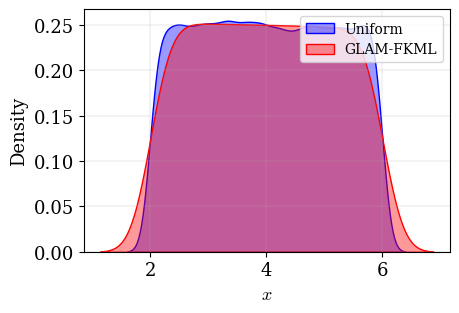
\includegraphics[width=\textwidth]{z_fig_uniform.png}
         \caption{Distribuição Uniforme}
         \label{fig:fit_uniform}
     \end{subfigure}
     \caption{Validação da capacidade de ajuste do PyGLAM para diferentes distribuições-alvo utilizando emuladores GLD.}
     \label{fig:pyglam_fits}
\end{figure}

\begin{table}[H]
\centering
\caption{Métricas quantitativas do ajuste GLD às distribuições-alvo. \falta{preencher}}
\label{tab:pyglam_metricas}
\begin{tabular}{lcccc}
\toprule
\textbf{Distribuição} & \textbf{$N$} & \textbf{Wasserstein} & \textbf{KS} & \textbf{Erro quantis P5/P50/P95 (\%)} \\
\midrule
Normal   & \faltanum & \faltanum & \faltanum & \faltanum \\
Gumbel   & \faltanum & \faltanum & \faltanum & \faltanum \\
Uniforme & \faltanum & \faltanum & \faltanum & \faltanum \\
\bottomrule
\end{tabular}
\end{table}

\subsection{Emulador global via Expansão em Caos Polinomial}
\label{subsec:pce}

Seguindo a metodologia proposta por \citet{ZhuSudret2021} e desenvolvimentos posteriores em metamodelagem estocástica, a GLD é acoplada à Expansão em Caos Polinomial (PCE) para a construção de um emulador global. Nesse arcabouço, a resposta estocástica do simulador para qualquer entrada $\mathbf{X}$ é modelada por uma GLD cujos parâmetros $\boldsymbol{\lambda}$ são, eles próprios, funções das variáveis de entrada.

Dado um conjunto de parâmetros de entrada $\mathbf{X}$ governado por uma função densidade de probabilidade conjunta $f_{\mathbf{X}}(\mathbf{x})$, cada componente do vetor de parâmetros $\lambda_i$ é aproximada por uma PCE truncada:

\begin{equation}
\lambda_i(\mathbf{X}) \approx \sum_{\boldsymbol{\alpha} \in \mathcal{A}} a_{i, \boldsymbol{\alpha}} \Psi_{\boldsymbol{\alpha}}(\mathbf{X}), \quad i = \{1, 2, 3, 4\}
\label{eq:pce_lambda}
\end{equation}

\noindent em que $\Psi_{\boldsymbol{\alpha}}(\mathbf{X})$ são polinômios ortonormais multivariados específicos das distribuições de entrada \citep{xiu2002}, $a_{i, \boldsymbol{\alpha}}$ são os coeficientes a determinar e $\mathcal{A}$ é o conjunto de multi-índices que define o esquema de truncamento (e.g., base de grau total) \citep{blatman2011}.

O procedimento de treinamento do emulador PCE--GLD segue os passos:

\begin{enumerate}
    \item \textbf{Plano de experimentos:} um conjunto de $M$ pontos amostrais $\{\mathbf{x}^{(1)}, \dots, \mathbf{x}^{(M)}\}$ é gerado por Amostragem por Hipercubo Latino (LHS) \citep{mckay1979}.
    \item \textbf{Avaliações estocásticas:} para cada ponto $\mathbf{x}^{(j)}$, o simulador estocástico original é executado $N$ vezes, gerando um conjunto amostral local da resposta, $\mathcal{Y}^{(j)}$.
    \item \textbf{Ajuste local da GLD:} o método dos momentos, implementado no PyGLAM com o otimizador BFGS, é utilizado para estimar os parâmetros locais ótimos $\hat{\boldsymbol{\lambda}}^{(j)}$ para cada $\mathcal{Y}^{(j)}$.
    \item \textbf{Estimação dos coeficientes da PCE:} a partir dos pares $\{\mathbf{x}^{(j)}, \hat{\boldsymbol{\lambda}}^{(j)}\}_{j=1}^M$, os coeficientes $a_{i, \boldsymbol{\alpha}}$ são calculados para cada $\lambda_i$.
\end{enumerate}

Uma vez treinado, o emulador fornece instantaneamente a distribuição de probabilidade completa (via parâmetros $\lambda$) para qualquer nova entrada $\mathbf{X}^*$, sem exigir novas execuções do simulador estocástico original.

\subsection{Emulação estocástica dependente do tempo}
\label{subsec:temporal}

O processo de carbonatação é inerentemente dependente do tempo, exigindo que a evolução da distribuição da margem de segurança seja capturada ao longo de toda a vida em serviço da estrutura. Para tanto, o arcabouço PCE--GLD é estendido para incluir o tempo $t$ como variável de entrada contínua. Nesse esquema de emulação temporal, os parâmetros $\boldsymbol{\lambda}$ da GLD são avaliados em passos de tempo discretos, e um metamodelo de aprendizado de máquina (ML) é subsequentemente treinado para mapear o espaço conjunto de variáveis físicas $\mathbf{X}$ e tempo $t$ nos parâmetros da distribuição.

A base de treinamento do emulador temporal é construída avaliando-se o simulador estocástico em $N_t$ passos de tempo discretos $\{t_1, t_2, \dots, t_{N_t}\}$ (e.g., 0, 10, 20, 50 e 80 anos). Para cada passo $t_m$, um conjunto de $M$ amostras do vetor de entrada $\mathbf{X}^{(j)}$ é avaliado, produzindo os parâmetros locais correspondentes $\hat{\boldsymbol{\lambda}}^{(j, m)}$ via PyGLAM. A base de dados resultante $\mathcal{D}$ é definida como:

\begin{equation}
\mathcal{D} = \left\{ \left( \mathbf{x}^{(j)}, t_m \right), \hat{\boldsymbol{\lambda}}^{(j, m)} \right\} \quad \text{para } j=1,\dots,M \text{ e } m=1,\dots,N_t
\label{eq:dataset_temporal}
\end{equation}

Para prever os parâmetros da GLD em um instante arbitrário $t^*$, emprega-se um modelo de ML de múltiplas saídas, que aprende o mapeamento não linear $f: (\mathbf{X}, t) \to \mathbb{R}^4$:

\begin{equation}
\hat{\boldsymbol{\lambda}}(\mathbf{X}, t) \approx \mathcal{M}_{ML}(\mathbf{X}, t; \mathbf{w})
\label{eq:ml_temporal}
\end{equation}

\noindent em que $\mathcal{M}_{ML}$ representa o regressor escolhido (e.g., florestas aleatórias, regressão por vetores de suporte ou redes neurais) e $\mathbf{w}$ denota os hiperparâmetros otimizados. Ao incluir o passo de tempo como entrada explícita, o emulador interpola os valores de $\{\lambda_1, \dots, \lambda_4\}$ entre os anos simulados, fornecendo uma evolução contínua da distribuição da margem de segurança ao longo de todo o período de análise. Duas salvaguardas são adotadas: (i) a restrição de validade $\lambda_2 > 0$ é imposta na saída do regressor por meio de \falta{descrever o mecanismo adotado: transformação $\log \lambda_2$, função de ativação positiva ou truncamento}; e (ii) parâmetros que exibam baixa sensibilidade às entradas podem ser excluídos do treinamento e representados por seu valor médio, decisão tomada caso a caso a partir de análise exploratória (ver Seção~\ref{subsec:exemplo1}).

\subsection{Métricas de validação do emulador}
\label{subsec:metricas}

A similaridade estatística entre os dados de referência (\textit{ground truth}, obtidos por simulação direta) e as amostras geradas pelo emulador é avaliada por um conjunto complementar de métricas, todas aplicadas em pontos e instantes \textit{não utilizados no treinamento}:

\paragraph{Testes de aderência.} O teste de Kolmogorov--Smirnov (KS) \citep{massey1951} quantifica a máxima distância entre as funções de distribuição acumuladas empíricas, sendo sensível a discrepâncias globais; o teste de Anderson--Darling (AD) \citep{anderson1952, scholz1987} pondera fortemente as caudas, sendo adequado para detectar desvios nas regiões extremas, justamente as mais relevantes para confiabilidade.

\paragraph{Comparação de quantis.} Erros relativos nos quantis $\{0{,}001;\, 0{,}01;\, 0{,}5;\, 0{,}99;\, 0{,}999\}$ localizam a origem de eventuais discrepâncias e quantificam diretamente a qualidade da aproximação na cauda inferior, região que governa a probabilidade de falha.

\paragraph{Divergência de Kullback--Leibler.} Para duas densidades $p(x)$ (referência) e $q(x)$ (emulador), a entropia relativa \citep{kullback1951, cover2006}

\begin{equation}
D(p \,\|\, q) = \int p(x)\, \log \frac{p(x)}{q(x)}\, dx
\label{eq:kl_continua}
\end{equation}

\noindent é não negativa e anula-se se, e somente se, $p = q$. Embora não seja simétrica nem satisfaça a desigualdade triangular, é frequentemente útil interpretá-la como uma medida de ``distância'' entre distribuições, fornecendo um escalar global de qualidade do emulador.
